%==========================================================
% PART 6: the control room (Phase 6).
%==========================================================
\par
% Phase 6 numbers, written by scripts/phase6/export_dashboard.py. Do not edit by hand.
\newcommand{\PsixAlgSites}{4,092}%
\newcommand{\PsixAlgLinks}{2,864}%
\newcommand{\PsixAlgFrames}{55}%
\newcommand{\PsixAlgCell}{31}%
\newcommand{\PsixAlgVertices}{312}%
\newcommand{\PsixAlgMb}{73}%
\newcommand{\PsixAlgTowerShare}{100}%
\newcommand{\PsixAlgPeakTruth}{62}%
\newcommand{\PsixAlgLeadAi}{-37}%
\newcommand{\PsixAlgLeadCl}{+16}%
\newcommand{\PsixAlgLeadSat}{-215}%
\newcommand{\PsixGhaSites}{220}%
\newcommand{\PsixGhaLinks}{153}%
\newcommand{\PsixGhaFrames}{85}%
\newcommand{\PsixGhaCell}{62}%
\newcommand{\PsixGhaVertices}{507}%
\newcommand{\PsixGhaMb}{160}%
\newcommand{\PsixGhaTowerShare}{5}%
\newcommand{\PsixGhaPeakTruth}{679}%
\newcommand{\PsixGhaLeadAi}{-87}%
\newcommand{\PsixGhaLeadCl}{+49}%
\newcommand{\PsixGhaLeadSat}{-123}%
\newcommand{\PsixTiles}{827}%

\clearpage
\begin{center}
\begin{minipage}{0.86\textwidth}
\small
\textbf{Part 6: one screen for the whole chain.} Parts 1 to 5 each answered one question: can a link measure rain, can
the AI do it better, can links make a map, would it work on Algerian towers, would it raise a flood alarm. A forecaster
on a stormy night has no time for five reports. They need one screen that shows, minute by minute, what the towers
measure, where the water goes, and whether to sound the alarm. This part describes that screen, how each piece of it is
drawn, and what it shows for the two storms. Same rules as before: every word explained, real numbers only, the
simulation clearly labelled.
\end{minipage}
\end{center}

\begin{careful}
\textbf{Still a simulation.} The screen replays the Part~4 storms and the Part~5 floods. The towers, terrain, buildings,
imagery and storms are real; the link signals, the true rain at 500\,m and the floods are simulated. A badge in the
corner of the screen says so at all times.
\end{careful}

%==========================================================
\section{What is on the screen}
\label{sec:p6_screen}
%==========================================================
The screen (Figure~\ref{fig:p6_screen}) is a 3D map of the city with panels around it. It is built like the flood
viewers used in research and by flood agencies: a 3D scene with a time slider, charts that move with the slider, and a
single status that says how worried to be.

\begin{figure}[h]
\centering
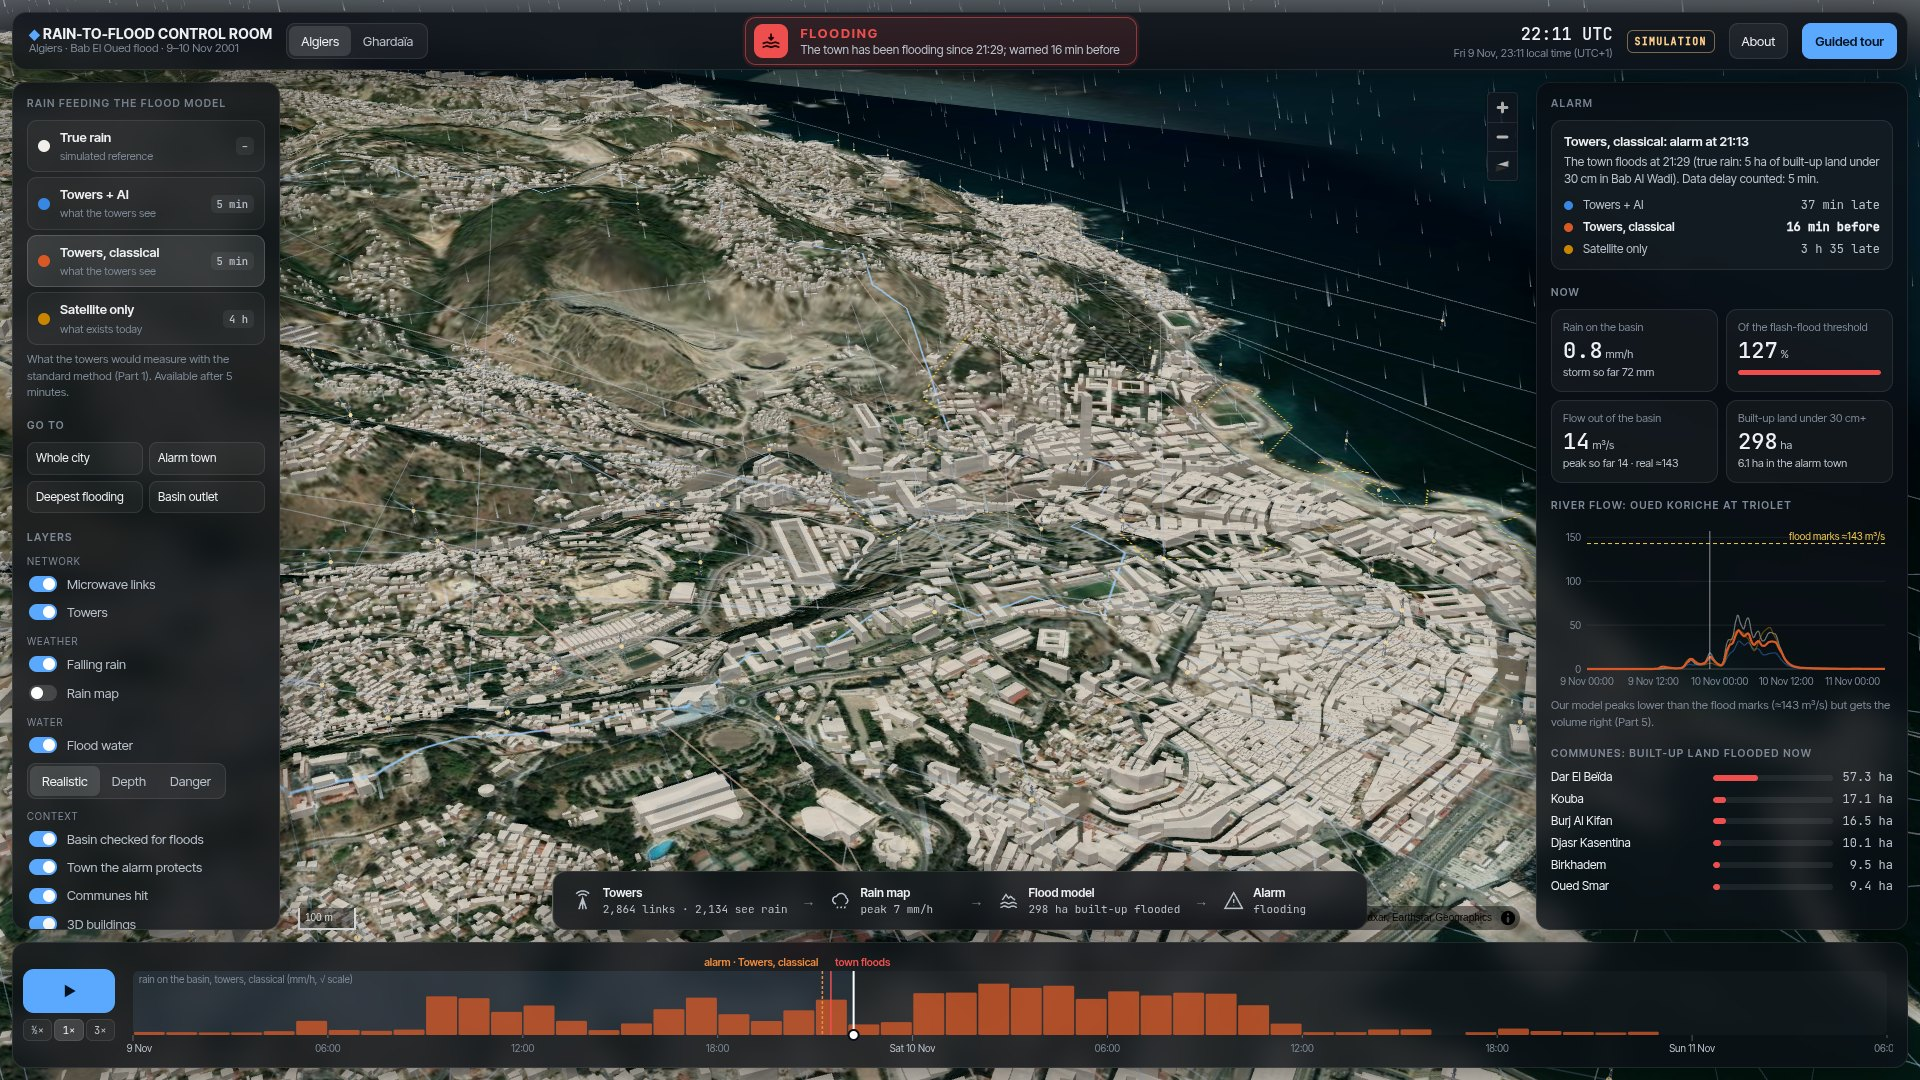
\includegraphics[width=\textwidth]{fig_p6_screen.jpg}
\caption{The control room during the 2001 storm, 42 minutes after Bab El Oued starts to flood, seen from above the Koriche
valley. Rain source: towers, read with the standard method. Left: the rain source and the layers. Centre: the city in 3D
with the towers, the links, the rain and the flood water. Right: the alarm, the figures of the moment, the flow out of the
basin, and the communes with flooded built-up land. Bottom: the chain from towers to alarm, and the timeline of the
storm.}
\label{fig:p6_screen}
\end{figure}

\begin{description}[leftmargin=0pt,itemsep=0.3em]
\item[The status, at the top.] One word and one colour, with an icon so it does not rely on colour alone:
\begin{itemize}
\item \textbf{normal}: rain below half of the flash-flood threshold (Section~\ref{sec:p5_warn});
\item \textbf{watch}: the rain over the town or the basin has reached half of the threshold;
\item \textbf{flood warning}: the flood model, run on the rain as it arrives, shows the town flooding;
\item \textbf{flooding}: the town is flooding (true rain: \PfiveAlgAlarmHa{}\,ha of built-up land under 30\,cm).
\end{itemize}
\item[The rain source, on the left.] The same storm, seen four ways: the simulated true rain; the towers read by the
AI; the towers read by the standard method; the satellite alone. Switching source changes everything on the screen:
the rain, the water, the figures and the alarm. This is the comparison of Part~5, made visible.
\item[The figures, on the right.] Rain on the basin now; how close the rain is to the flash-flood threshold; the flow
out of the basin (with the value engineers estimated from flood marks); built-up land under 30\,cm of water; and the
communes with the most flooded built-up land at that moment.
\item[The chain, at the bottom.] Four boxes, \emph{Towers $\rightarrow$ Rain map $\rightarrow$ Flood model $\rightarrow$
Alarm}, each with its live number: how many links see rain, the heaviest rain on the map, the flooded built-up land,
and the status. Clicking a box flies the camera to the place that box is about.
\item[The timeline.] The rain on the basin hour by hour, with two marks: when this rain source raises the alarm, and
when the town floods. Press play, or drag.
\end{description}

%==========================================================
\section{How each piece is drawn}
\label{sec:p6_drawing}
%==========================================================
\textbf{The ground.} The 3D terrain is made from the very same elevation map the flood model used (Copernicus GLO-30,
\PsixTiles{} map tiles for both cities). This matters: if the map's hills and the model's hills differ by a few metres,
water floats in the air or disappears under the ground. On top of it: satellite imagery (Esri) and buildings from
OpenStreetMap, raised to their height.

\textbf{The towers and links.} The \PsixAlgSites{} real tower sites of Algiers and the \PsixAlgLinks{} simulated links of
Part~4. A link is drawn between the dishes of its two towers. It turns from blue to orange as its rain grows, and it
shows what that link \emph{measured} with the chosen source, not the true rain.

\textbf{The water.} This is the heart of the screen. For it we re-ran the Part~5 flood model with one change: it saves
the water every hour at full detail (\PsixAlgCell\,m squares in Algiers, \PsixGhaCell\,m in Ghardaïa), including how
fast and in which direction it moves. The rerun gives exactly the same flow as Part~5 (the largest difference, at any
minute, is zero). The screen then turns these hours into a moving water surface:
\begin{itemize}
\item a surface of \PsixAlgVertices{} thousand points in Algiers (\PsixGhaVertices{} thousand in Ghardaïa), placed on every
square that is ever wet, raised by the water depth;
\item between two saved hours the depth is blended smoothly, so the flood rises and falls instead of jumping;
\item water thinner than 3\,cm is not drawn, and the edges fade out instead of ending in squares.
\end{itemize}
Three ways to colour it (Figure~\ref{fig:p6_water}):
\begin{itemize}
\item \textbf{Realistic}: muddy brown, darker where deeper, with the grey of the storm sky reflected on it. Small ripples
drift in the direction the model says the water flows, white streaks show where it runs fast, and rain dimples the
surface while it rains. Seen from far away, flooded ground looks like a silver sheet, as it does in aerial photos.
\item \textbf{Depth}: the blue scale of Part~5, from 3\,cm to 2\,m and more.
\item \textbf{Danger}: the hazard rating of Part~5, depth $\times$ (speed $+\,0.5$) plus debris, in four classes.
\end{itemize}

\begin{figure}[h]
\centering
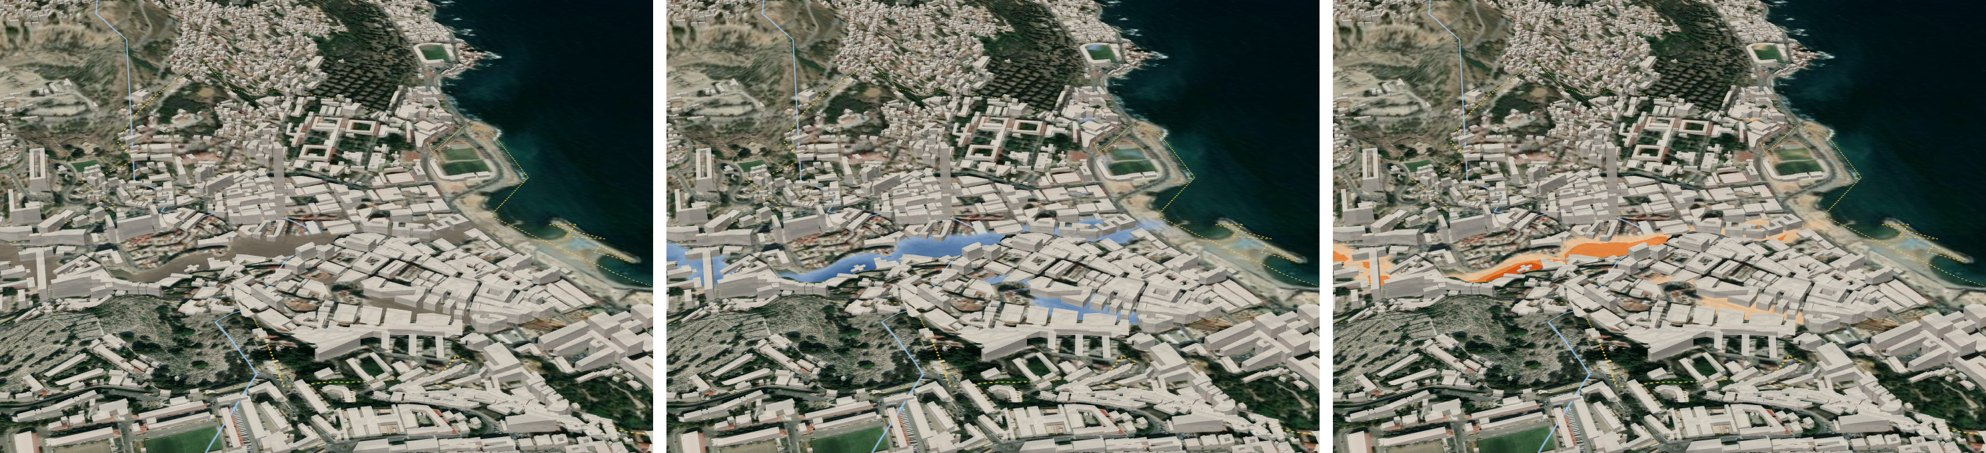
\includegraphics[width=\textwidth]{fig_p6_water.jpg}
\caption{Bab El Oued at the same moment, three ways. Left: realistic. Middle: depth. Right: danger to people. The flood runs
down the main avenue of the valley to the sea, where the 2001 flood went. Buildings hide the water behind them, as they
should.}
\label{fig:p6_water}
\end{figure}

\textbf{The rain.} Falling rain is drawn as streaks that lean with the wind, more of them where the chosen rain map is
heavier; they fade out when the camera is far away, where they would look like dust. The sky darkens and the imagery
greys as the true storm grows. An optional layer drapes the rain map itself on the ground, one colour per 500\,m
square.

%==========================================================
\section{A guided tour}
\label{sec:p6_tour}
%==========================================================
For people who see the screen for the first time (judges, a mayor, a journalist), a \emph{Guided tour} button walks
through the chain in seven steps for Algiers and three for Ghardaïa. Each step moves the clock, flies the camera, switches
the layers it needs and lights up its box in the chain:
\begin{enumerate}
\item the links over the city before the storm;
\item the storm arriving, the links warming from blue to orange;
\item the rain map the AI makes from the links alone;
\item the water gathering in the Koriche valley and running down to Bab El Oued;
\item the alarm, in minutes before the town floods: \PsixAlgLeadCl{} with towers read by the standard method,
\PsixAlgLeadAi{} with the AI and \PsixAlgLeadSat{} with the satellite (a minus sign means after the flood started);
\item the danger map and the communes hit;
\item the same storm with the satellite only, which is what exists today.
\end{enumerate}
The Ghardaïa tour shows the honest limit of the idea (Figure~\ref{fig:p6_ghardaia}): the dashed box where tower rain
exists covers only \PsixGhaTowerShare\% of the 1{,}387\,km\textsuperscript{2} basin. The flood comes from rain that falls
far upstream, where there are no towers.

\begin{figure}[h]
\centering
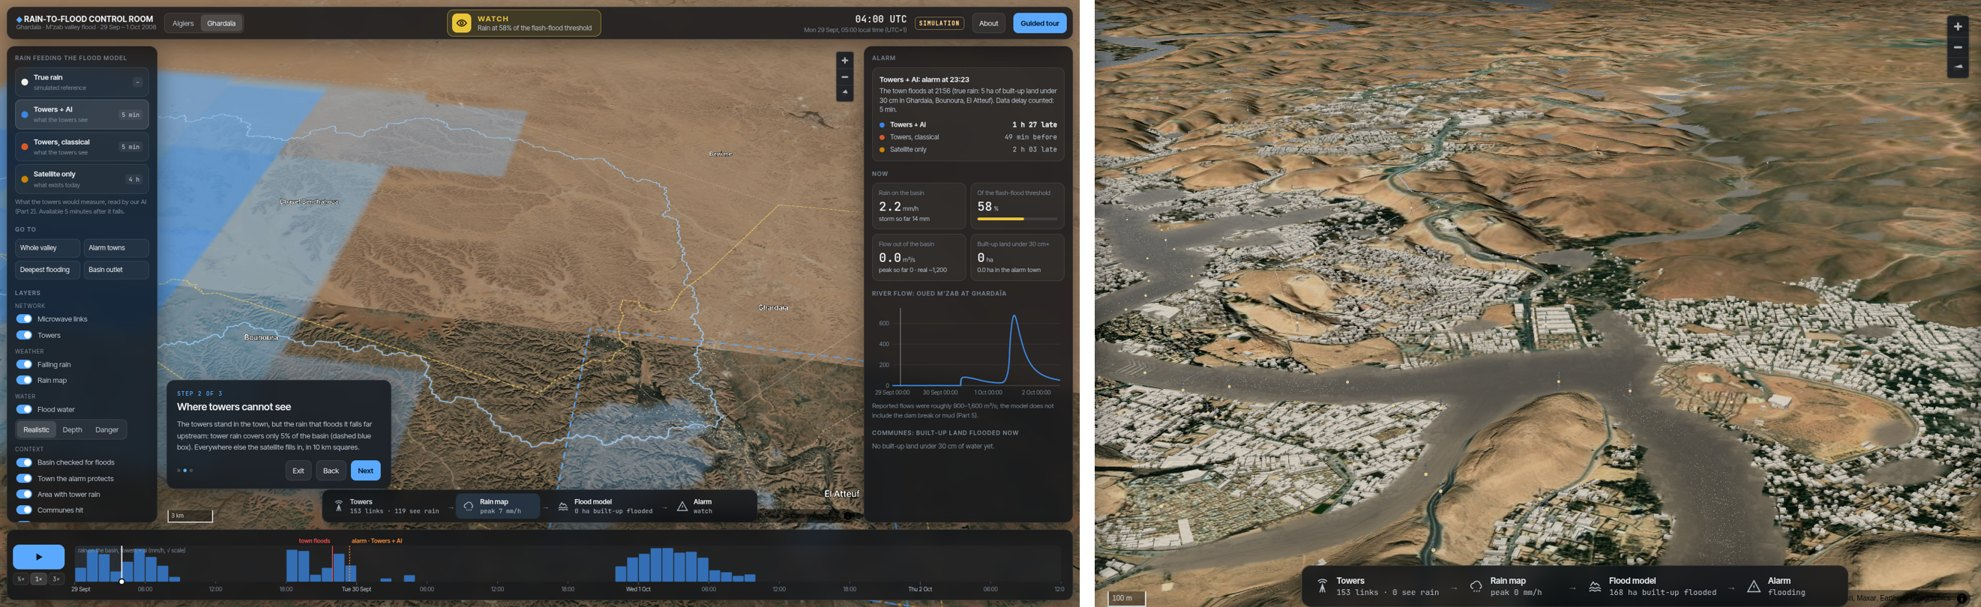
\includegraphics[width=\textwidth]{fig_p6_ghardaia.jpg}
\caption{Ghardaïa. Left: step 2 of the tour. The rain map from towers covers only the small dashed box around the town;
the rest of the basin (white outline) gets the satellite's 10\,km squares. Right: the M'zab wadi at its peak flow
(\PsixGhaPeakTruth\,m\textsuperscript{3}/s with the true rain), flooding through the town between the desert hills.}
\label{fig:p6_ghardaia}
\end{figure}

%==========================================================
\section{What the screen shows, in numbers}
\label{sec:p6_numbers}
%==========================================================
Nothing new is computed for the screen: every number comes from the Part~5 runs. But putting them side by side, on a
clock, makes the point of the whole project easy to see.

\begin{center}\small
\begin{tabular}{lrr}
\toprule
Minutes between the alarm and the town flooding (positive: in time) & Algiers & Ghardaïa\\
\midrule
Towers, standard method & \PsixAlgLeadCl & \PsixGhaLeadCl\\
Towers + AI & \PsixAlgLeadAi & \PsixGhaLeadAi\\
Satellite only (4\,h data delay) & \PsixAlgLeadSat & \PsixGhaLeadSat\\
\bottomrule
\end{tabular}
\end{center}

\begin{itemize}
\item \textbf{The satellite is always late}, by two to four hours, because its first estimate is published about four
hours after the rain. Today that is the only rain map that covers all of Algeria.
\item \textbf{Tower rain read with the standard method warns in time} in both storms. In Ghardaïa this works although the
towers cover a twentieth of the basin: when the town starts to flood in the model, the flow coming down the M'zab is still
small (the timeline and the flow chart show it), so it is the rain on the town itself that floods it first, and that
rain the towers do see. The big wadi flood, about a day and a half later, comes from upstream.
\item \textbf{Tower rain read by the AI is late} in both storms. This is the AI's known weakness from Part~2: it measures
too little heavy rain, so its flood comes later and smaller. It is the first thing to fix (Part~2, Section~18).
\end{itemize}

\begin{oneline}
One screen now runs the whole chain on real Algerian towers, terrain and storms: links that light up with rain, a rain
map, water that rises in the right streets and the alarm that follows. It makes the main result of the project visible
at a glance: tower rain arrives hours before the satellite's, but the AI must stop under-measuring heavy rain before its
alarms can be trusted.
\end{oneline}

%==========================================================
\section{Every choice, and why}
\label{sec:p6_choices}
%==========================================================
\begin{center}\footnotesize\setlength{\tabcolsep}{4pt}
\begin{tabular}{>{\raggedright\arraybackslash}p{2.8cm}>{\raggedright\arraybackslash}p{3.6cm}>{\raggedright\arraybackslash}p{6.9cm}}
\toprule
Choice & Value & Why\\
\midrule
Map engine & MapLibre GL and deck.gl & free, open, run in any browser; the same engines as GeoLibre and many flood viewers\\
Terrain & the flood model's own DEM & water and ground must agree to the metre\\
Water frames & every hour, full detail, with speed & enough for smooth blending; \PsixAlgMb\,MB (Algiers) and \PsixGhaMb\,MB
(Ghardaïa) of data, loaded only for the chosen source\\
Water drawing & a custom GPU shader & depth colour, sky reflection, ripples that follow the flow; nothing ready-made does
this for model output\\
Storm version & gauge-matched only & the real flood's strength; the satellite-strength version stays on the Part~5 page\\
Status levels & normal / watch / warning / flooding & the usual flash-flood ladder; watch at half the threshold\\
Alarm & the flood model on the arriving rain & the alarm of Part~5, with the same data delays (towers 5\,min, satellite
4\,h)\\
Colours & fixed per rain source; status colours reserved & the same source keeps the same colour on every panel, and
status colours always come with an icon and a word\\
Tour & 7 + 3 steps, numbers filled from the data & the story is told by the data, so it stays true if the runs change\\
\bottomrule
\end{tabular}
\end{center}

\textbf{How to open it.} On the project computer, \texttt{python scripts/serve\_site.py} serves the site; the control room
is at \texttt{/dashboard/}. It needs internet for the imagery and the buildings; everything else is local. It also works
on a phone, with the panels stacked under the map.

\textbf{Next:} Part~7 takes the same chain off the replay and runs it live, on any city.
